%%%%%%%%%%%%%%%%%%%%%%%%%%%%%%%%%%%%%%%%%
% Dreuw & Deselaer's Poster
% LaTeX Template
% Version 1.0 (11/04/13)
%
% Created by:
% Philippe Dreuw and Thomas Deselaers
% http://www-i6.informatik.rwth-aachen.de/~dreuw/latexbeamerposter.php
%
% This template has been downloaded from:
% http://www.LaTeXTemplates.com
%
% License:
% CC BY-NC-SA 3.0 (http://creativecommons.org/licenses/by-nc-sa/3.0/)
%
%%%%%%%%%%%%%%%%%%%%%%%%%%%%%%%%%%%%%%%%%

%------------------------------------------------------------------------------
%	PACKAGES AND OTHER DOCUMENT CONFIGURATIONS
%------------------------------------------------------------------------------

\documentclass[final,hyperref={pdfpagelabels=false}]{beamer}

\usepackage{soul}

\usepackage[firstinits=true,backend=bibtex,doi=false,isbn=false,url=false,maxnames=1]{biblatex}
\AtEveryBibitem{%
  \clearfield{pages}%
}
\renewcommand{\bibfont}{\normalfont\footnotesize}
\addbibresource{bib.bib}

\usepackage[orientation=portrait,size=a0,scale=1.4]{beamerposter} % Use the beamerposter package for laying out the poster with a portrait orientation and an a0 paper size

\usetheme{I6pd2} % Use the I6pd2 theme supplied with this template

\usepackage[english]{babel} % English language/hyphenation
\usepackage{graphicx}
\usepackage{amsmath,amsthm,amssymb,latexsym} % For including math equations, theorems, symbols, etc

%\usepackage{times}\usefonttheme{professionalfonts}  % Uncomment to use Times as the main font
%\usefonttheme[onlymath]{serif} % Uncomment to use a Serif font within math environments

\boldmath % Use bold for everything within the math environment

\usepackage{booktabs} % Top and bottom rules for tables

\graphicspath{{figures/}} % Location of the graphics files

\usecaptiontemplate{\small\structure{\insertcaptionname~\insertcaptionnumber: }\insertcaption} % A fix for figure numbering

%------------------------------------------------------------------------------
%	TITLE SECTION 
%------------------------------------------------------------------------------

\title{\LARGE Does Connectivity Control Lake Phosphorus Retention?} % Poster title

\author{Joseph Stachelek, Pat Soranno} % Author(s)

\institute{Department of Fisheries and Wildlife, Michigan State University, MI, USA} % Institution(s)

%------------------------------------------------------------------------------
%	FOOTER TEXT
%------------------------------------------------------------------------------

\newcommand{\leftfoot}{https://jsta.rbind.io} % Left footer text

\newcommand{\rightfoot}{stachel2@msu.edu} % Right footer text

%------------------------------------------------------------------------------
\usepackage{pgfplots}
\input{../../../../tex/beamer-lake-fig/beamer-lake-fig.tex}
\begin{document}

\addtobeamertemplate{block end}{}{\vspace*{2ex}} % White space under blocks

\begin{frame}[t] % The whole poster is enclosed in one beamer frame
\vspace{1em}
\begin{columns}[t] % The whole poster consists of two major columns, each of which can be subdivided further with another \begin{columns} block - the [t] argument aligns each column's content to the top

\begin{column}{.02\textwidth}\end{column} % Empty spacer column

\begin{column}{.465\textwidth} % The first column

%------------------------------------------------------------------------------
%	INTRODUCTION
%------------------------------------------------------------------------------
            
\begin{block}{Introduction}

\begin{itemize}
% \item A comprehensive understanding of phosphorus (P) cycling is neccessary to predict P concentrations among many different lakes types and to better manage the risk of eutrophication from excess nutrient loading.
% \vspace{1em}
% \item P retention is a desirable metric for assessing eutrophication risk because it is a unitless measure that can be easily compared among different lake types irrespective of their baseline P concentrations or total P inputs.
% \vspace{1em}
% \item P retention is typically modelled as a function of a given lake's volume-weighted hydrologic flux (or its inverse, \alert{residence time}).
% \vspace{-0.5em}
\item There is some evidence that P retention in lakes and streams is affected by network connectivity:
\end{itemize}

\vspace{1em}
{
\setbeamercolor{block title}{fg=black,bg=orange!70} % Change the block title color
\setbeamercolor{block body}{bg=white}
\begin{beamercolorbox}[wd=\textwidth,rounded=true]{block body}
   \begin{figure}
      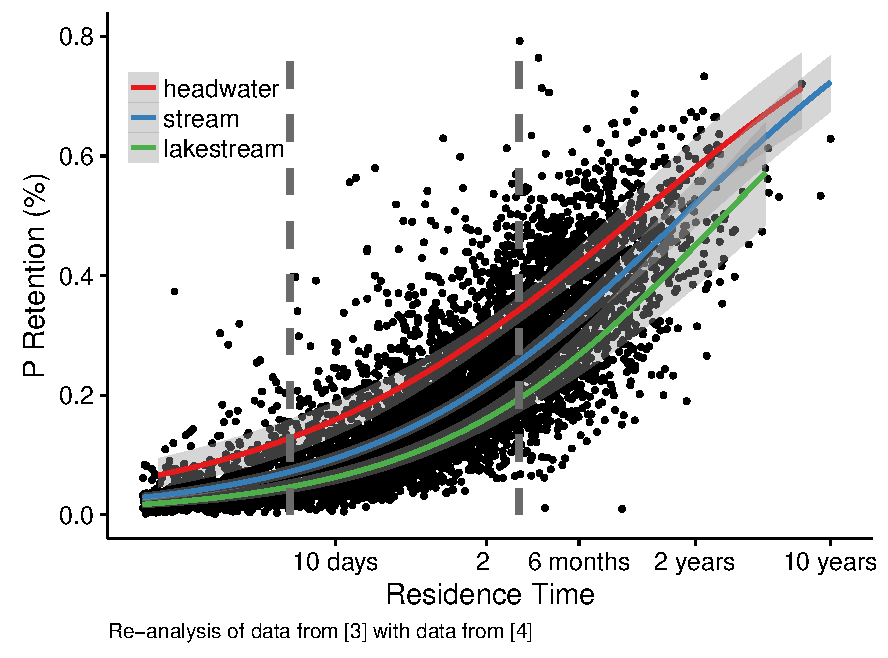
\includegraphics[width=\linewidth]{milstead_multi.pdf}
   \end{figure}
\end{beamercolorbox}
}

\vspace{1.4em}

\begin{columns}

\begin{column}{0.5\textwidth}
\centering
\large stream \\
\vspace{0.5em}
\primaryprofileflatequal[1.5]{white} \\
\textbf{Less Connected}
\end{column}

\begin{column}{0.5\textwidth}
\centering
\large lakestream \\
\vspace{0.5em}
\secondaryprofileflatequal[1.5]{white} \\
\textbf{More Connected}
\end{column}
\end{columns}
\vspace{0.3em}

\vspace{0.5em}
\end{block}
%------------------------------------------------------------------------------
%	Research Questions
%------------------------------------------------------------------------------
\vspace{1em}
\begin{block}{Research Questions}

\begin{enumerate} \large 
\item \textbf{Do connected lakes retain less P than less connected lakes (given equal residence times)?}
\vspace{1em}
\item \textbf{Are there differences in the relative influence of biological and hydrological control on P retention in lakes of differing connectivity?}
\end{enumerate}

\vspace{1em}
{
\setbeamercolor{block title}{fg=black,bg=orange!70} % Change the block title color
\setbeamercolor{block body}{bg=white}
\begin{beamercolorbox}[wd=\textwidth,rounded=true]{block body}

\begin{figure}
  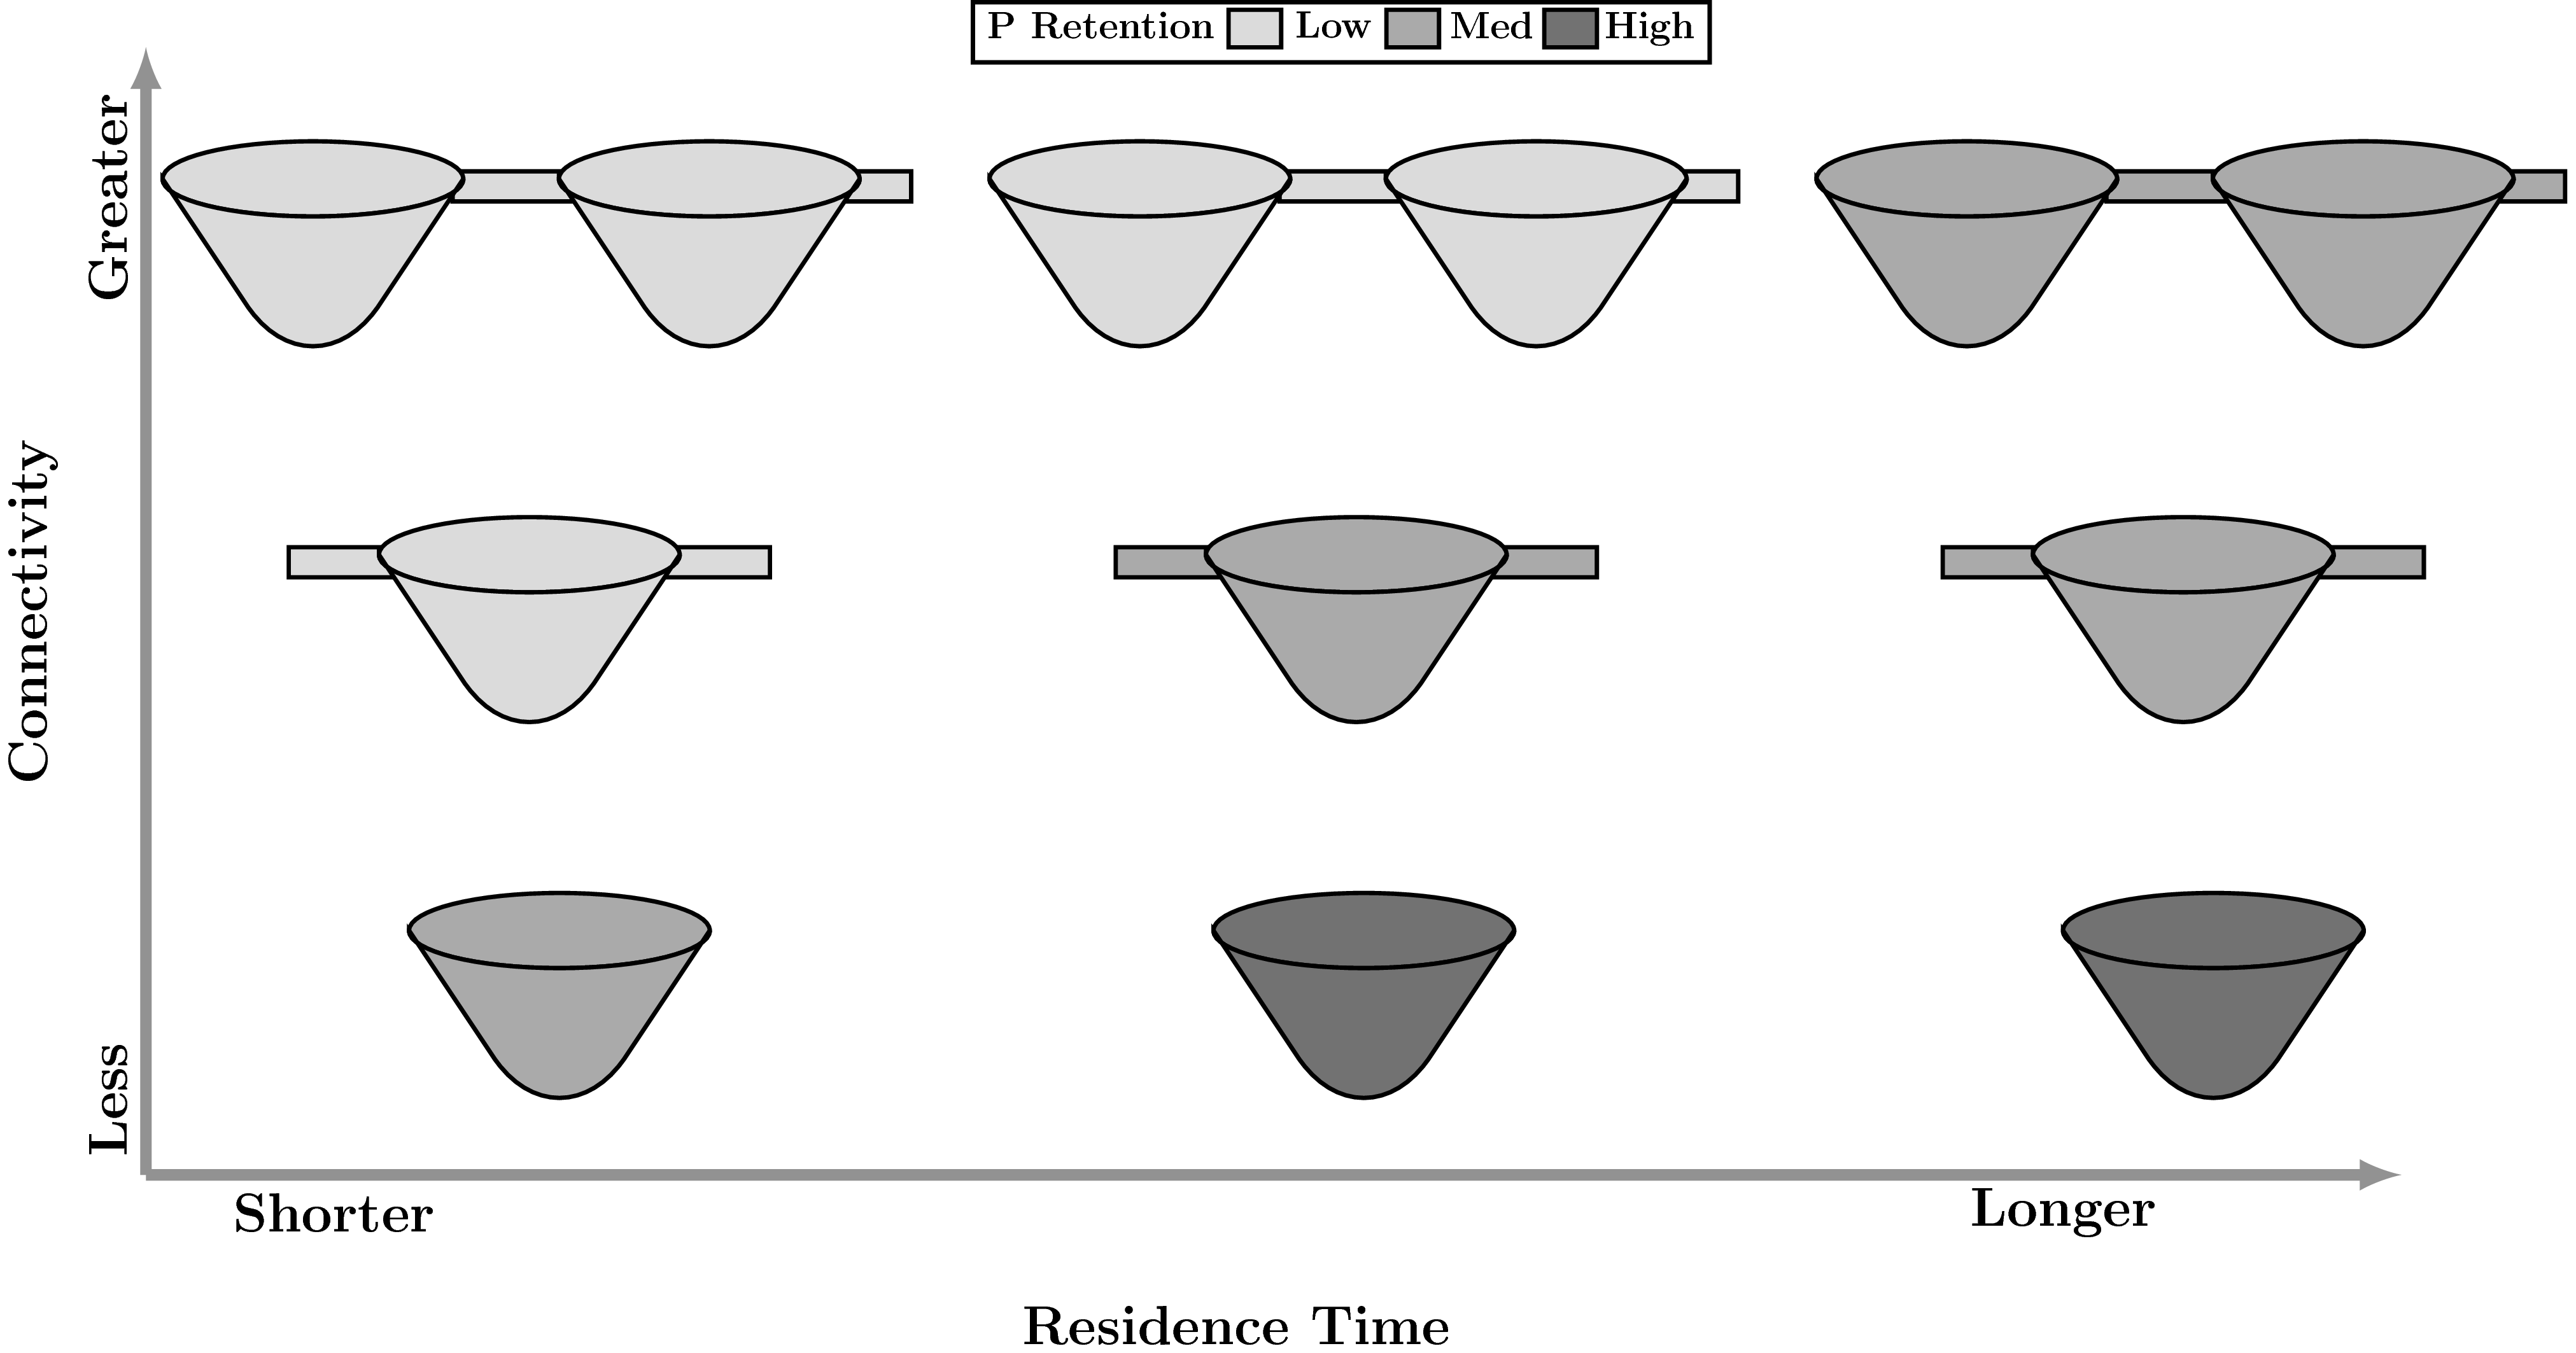
\includegraphics[width=\linewidth]{conny_framework.pdf}
\end{figure}

\end{beamercolorbox}
}
\vspace{0.5em}
\end{block}

%------------------------------------------------------------------------------

\vspace{1em}

\begin{block}{Methods}

\begin{itemize}
\item Data on P loading, P export, and residence time from approximately 250 lakes included in the National Eutrophication Survey (1972 - 1975)\cite{StachelekNationalEutrophicationSurvey2017}.
\end{itemize}

\end{block}

\end{column} % End of the first column

\begin{column}{.03\textwidth}\end{column} % Empty spacer column
 
\begin{column}{.465\textwidth} % The second column

%------------------------------------------------------------------------------
%	METHODS
%------------------------------------------------------------------------------
\begin{block}{Methods Con't}

\begin{itemize}
\item Model P retention as a function of residence time using 2 parameter ($k$, $x$) Vollenweider models \cite{Brettreviewreassessmentlake2007}. 
\vspace{1em}
\item $k$ (removal rate coefficient) and $x$ (hydrologic flux coefficient) can be interpreted as representing biological and hydrological controls on P retention respectively.

% \item Lakes were sampled on a monthly basis for a one year period in one of 1972, 1973, 1974, or 1975.
% \item P loads were estimated as the sum of the loads contributed by incoming tributaries.
% \item Retention time was computed on the basis of concurrent USGS gage measurements normalized to estimate a mean flow for each month in an average year.
% \item P retention was computed using a modification of the Vollenweider equations (see under flap, \cite{Brettreviewreassessmentlake2007}).
\end{itemize}

% \begin{column}{.43\textwidth} % The second subdivided column within the first main column
% \centering
% \begin{figure}
% 
\includegraphics[width=0.8\linewidth]{placeholder.jpg}
% \caption{Figure caption}
% \end{figure}
% \end{column}

\end{block}

% {
% \setbeamercolor{block title}{fg=black,bg=orange!70} % Change the block title color
% \setbeamercolor{block body}{bg=white}
% \begin{beamercolorbox}[wd=\textwidth,rounded=true]{block body}
% 
% \begin{equation*}
% P\, Retention \sim k, x
% \end{equation*}
% 
% \begin{equation*}
% \begin{split}
% k \sim Connectivity\, Type
% \end{split}
% \end{equation*}
% 
% \end{beamercolorbox}
% }

\vspace{1em}

%------------------------------------------------------------------------------
%	RESULTS
%------------------------------------------------------------------------------
\begin{block}{Results}
\begin{enumerate}
\item \textbf{No, lakes with and without upstream lakes had similar distributions of residence time and P retention.}
\vspace{1em}
\item \textbf{Yes, estimates of the removal rate coefficient ($k$) were higher in (less connected) lakes without upstream lakes.}
\end{enumerate}
\vspace{1em}
\large \textbf{\ul{This suggests that P inputs are controlled by biological processes to a greater extent in lakes without upstream lakes.}}

\vspace{1em}
{
\setbeamercolor{block title}{fg=black,bg=orange!70} % Change the block title color
\setbeamercolor{block body}{bg=white}
\begin{beamercolorbox}[wd=\textwidth,rounded=true]{block body}

\begin{figure}
  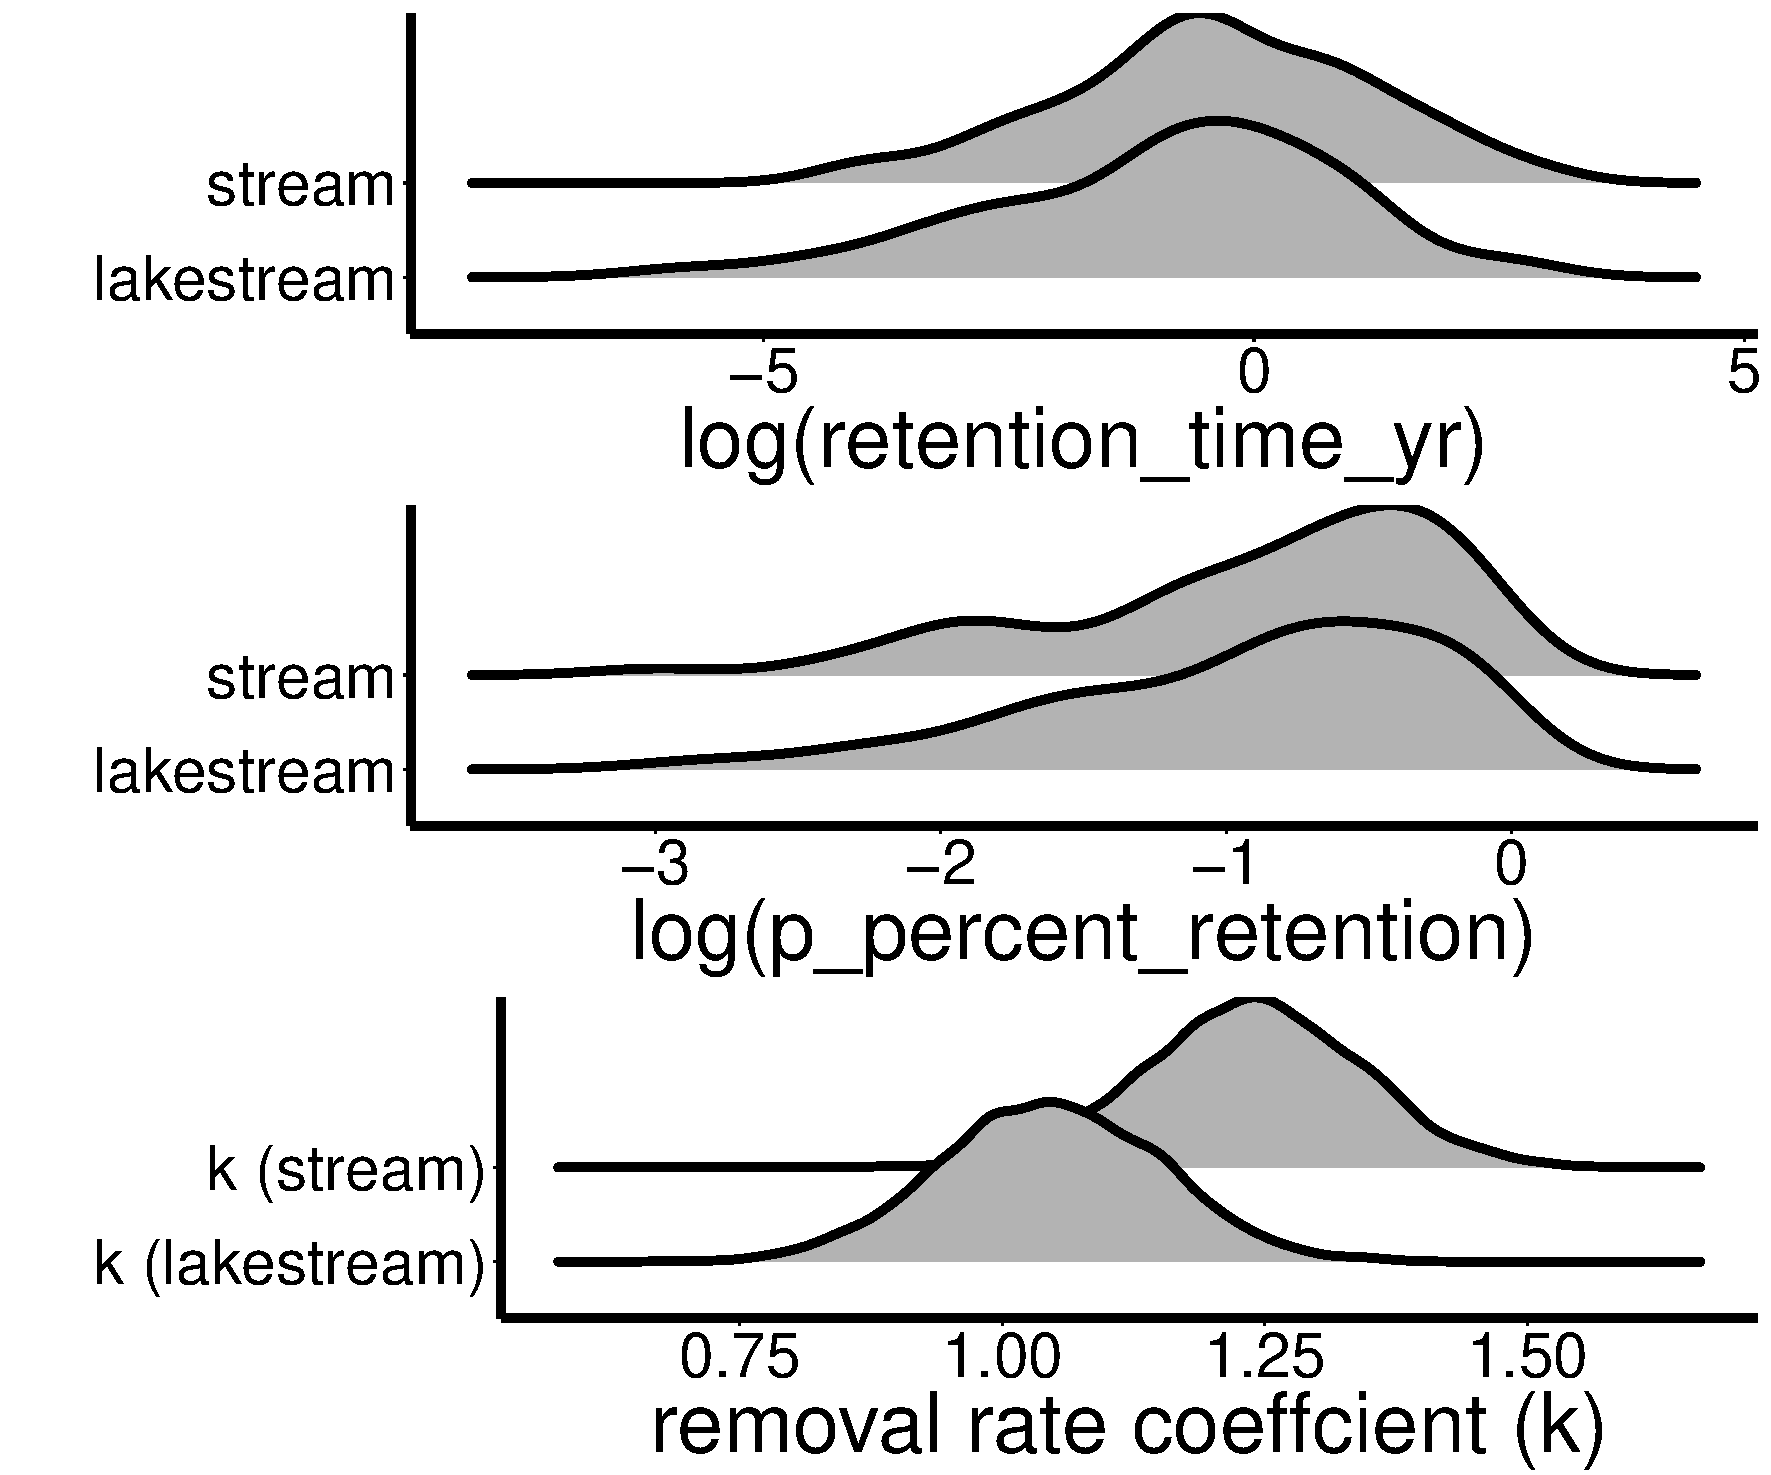
\includegraphics[width=30cm]{gleon_poster.pdf}
\end{figure}

\end{beamercolorbox}
}
\vspace{0.5em}
\end{block}

%------------------------------------------------

\vspace{0.8em}

%------------------------------------------------------------------------------
%	FUTURE WORK
%------------------------------------------------------------------------------
\begin{block}{Future Work}

\begin{itemize}
\item Calculate network properties of each lake catchment such as stream density, upstream lake area, average link length, and stream order ratio.
\vspace{1em}
\item Model $k$ and $x$ seperately via 2-component hierarchical models that relate P retention to \textbf{lake catchment network properties} as well as other potential explanatory factors such as landuse and climate.
\end{itemize}
\end{block}


%------------------------------------------------------------------------------
%	REFERENCES
%------------------------------------------------------------------------------
\vspace{1em}

\begin{block}{References}

\nocite{*}
\begingroup
\setlength\bibitemsep{0pt}
\setlength\bibnamesep{0pt}
\printbibliography[heading=none]
\endgroup
\end{block}

\begin{tabular}{cc}

\raisebox{-0.5\height}{\includegraphics[width=5cm]{nsf2.pdf}} & \raisebox{-\height}{\small Viginia Tech - NSF \#1517823}
\end{tabular}

%------------------------------------------------------------------------------

\end{column} % End of the second column

\begin{column}{.015\textwidth}\end{column} % Empty spacer column

\end{columns} % End of all the columns in the poster

\end{frame} % End of the enclosing frame

\end{document}